%%%%%%%%%%%%%%%%%%%%%%% file template.tex %%%%%%%%%%%%%%%%%%%%%%%%%
% $Id: icad-example.tex 163 2017-05-15 23:02:51Z foley $
% $URL: https://repository.cs.ru.is/svn/template/tvd/journal/matec-woc/icad-example.tex $
% 
% This is a template file for Web of Conferences Journal
%
% Copy it to a new file with a new name and use it as the basis
% for your article
%
% This template has been updated to match the Word Template's contents
% by Joseph T. Foley < foley AT RU dot IS >
%
%%%%%%%%%%%%%%%%%%%%%%%%%% EDP Science %%%%%%%%%%%%%%%%%%%%%%%%%%%%
%
%%%\documentclass[option]{webofc}
%%% "twocolumn" for typesetting an article in two columns format (default one column)
%
\documentclass[twocolumn]{webofc}
\usepackage[varg]{txfonts}   % Web of Conferences font
\usepackage{booktabs}
\usepackage{array} %% needed for advanced table manipulation
%% Column types from http://tex.stackexchange.com/questions/54069/table-with-text-wrapping
\newcolumntype{L}[1]{>{\raggedright\let\newline\\\arraybackslash\hspace{0pt}}m{#1}}
\newcolumntype{C}[1]{>{\centering\let\newline\\\arraybackslash\hspace{0pt}}m{#1}}
\newcolumntype{R}[1]{>{\raggedleft\let\newline\\\arraybackslash\hspace{0pt}}m{#1}}

\graphicspath{{graphics/}{Graphics/}}  % where to look for graphics
%
% Put packages and macros that you use often in custom.sty
\usepackage{custom}

%% Fixmes are reminders of things that still need to be done.
%% The default fixmes are:  \fxnote{} \fxwarning{} \fxerror{} \fxfatal{} (same as \fixme{})
% if you want personalized fixmes, then register the authors here
% notice that the first field is 2 letters, the second is 3.
\FXRegisterAuthor{jf}{jtf}{foley}
% this registers \jfnote{}, \jfwarning{}, \jferror{}, \jffatal{}

\begin{document}
        %
        \title{International Conference of Axiomatic Design 2019 Template: MATEC Web of Conferences}
        %
        % subtitle is optionnal
        %
        %%%\subtitle{Do you have a subtitle?\\ If so, write it here}

        \author{\firstname{Emilía Tinna} \lastname{Sigurðardóttir}\inst{1}
        ,
  \firstname{Erla} \lastname{Sigurjónsdóttir}\inst{1}
  ,
  \firstname{Hekla Bryndís} \lastname{Jóhannsdóttir}\inst{1} \and \firstname{Sóley Sara} \lastname{Eiríksdóttir}\inst{1}
  % etc.
}

\institute{
  Department of Science and Engineering. Reykjavik University, Menntavegur 1, Reykjavik 101, Iceland
}

\abstract{%
        Many pet owners struggle with feeding their pets while away for a long time. They worry about bothering their friends and family to constantly check on their pet and feed them. This project employs the Axiomatic Design method to build an automatic pet feeder with a weight sensor that indicates the amount of food the pet has eaten which facilitates tracking the pet's food consumption. The feeder can be controlled manually via WiFi either on a computer or phone. Owners can also choose to automate the feeder in such a way that when the weight in the bowl goes below a certain weight the feeder turns on. This way owners can take vacations, carefree, and at the same time monitor their pet's intake.
}
%
\maketitle
%
\listoffixmes{}

\section{Introduction}
\jfnote{Don't forget to write the introduction.}
\jfwarning{Really, don't forget to write the introduction.}
People live busy lives today and something can easily be forgotten in the daily routine.
An example of an important task in many people’s daily lives, that is often forgotten, is feeding their pet.

When a person goes on vacation, they must find someone to come feed the pet.
This can be a hassle and it’s not always guaranteed the pet-sitter will remember to come by every day.

The goal of this project is to make an automatic pet feeder that will make sure the pet always has enough food.
If an owner forgets to feed their pet before leaving the house or is on a vacation and can’t physically perform the task, they don’t have to worry about their pet starving.
They can relax without guilt knowing that the pet is always taken care of. 

\subsection{Customer Needs}
Following the principles of the Axiomatic Design theory, the first step is defining the Customer Needs(CN)~\cite{suh1990principles}.
After communicating with pet owners about their needs it became clear that they wish to be able to feed their pets while away in an easy and affordable manner.
The top-level need \CN0 becomes:
\begin{quote} \textbf{\CN0} The pet owner needs to be able to feed their pet while away or if they forget and have left the house.
\end{quote}
Lower CAs were determined to be:
\begin{quote} \textbf{\CN1} The pet needs to be fed.
\end{quote}
\begin{quote} \textbf{\CN2} The owner needs to be able to tell if the pet eats while they are away.
\end{quote}
\begin{quote} \textbf{\CN3} Need to be able to ration the amount of food the pet gets.
\end{quote}
\begin{quote} \textbf{\CN4} Wanting to avoid asking friends and family to come in and feed the pet.
\end{quote}





\section{Backround}
Most people conventionally pour the pet food manually into a bowl.
It’s not a new concept to automate this process and other companies have come out with their own products to fulfill this need.
However, there is no such product available in Iceland.

In order to get an automated food dispenser, the customer must order it online.
This can be tricky because when ordering electronics from outside the EU the customer needs to make sure it has been certified according to EU health and safety standards like the CE mark~\cite{CE_mark}.

Voltages also differ around the world and electronics ordered, for example, from the USA will not work in Iceland without an adapter~\cite{adapters_outlets}.

Looking at these points, there is a clear advantage in offering a product like this in Iceland. From the seller's point of view, there is no local competition and the customer wins because they don't have to pay shipping or customs fees and the product gets delivered immediately. 

~\subsection{Available products}
It’s worth looking at competing products to see how they compare to this project.

The intelligent food dispenser by OHANA can be seen in Fig. 1.
The product has a camera and a speaker that connects to a mobile app that can be used to check in on the pet or even talk to it.
It also has a weighing mechanism and a timer so the user can time the feedings and the amount given.~\cite{ohana_dispenser}

The Automatic Dog and Cat Feeder by PetSafe, seen in Fig. 2, is simpler in its design. 
There is a timer so the user can schedule the feeds, by using buttons on the machine, and different settings for how the food should be dispensed.
The “slow feed” setting helps slow down eager eaters as the food is dispensed over a longer period.
“Immediate feed” releases food, as the name suggests, immediately. The “pause feed” stops the dispenser without losing schedule.
It can dispense from 29ml up to 940ml of food depending on what the user chooses.~\cite{pet_safe}


\subsection{Functional Requirements}
Still following the principles of the Axiomatic Design theory, the second step is looking at the CNs and translating them into Functional Requirements (FR)~\cite{suh1990principles}.
The top-level primary \textbf{\FR0} was determined to be an “Automated food dispense system that is user-controlled”.

\begin{quote} \textbf{\FR1} Delivers food.
\end{quote}
\begin{quote} \textbf{\FR2} Dispensed food can be weighed.
\end{quote}
\begin{quote} \textbf{\FR3} Reliable and constant power.
\end{quote}
\begin{quote} \textbf{\FR4} Controllable when absent.
\end{quote}


\begin{figure}
  \centering
  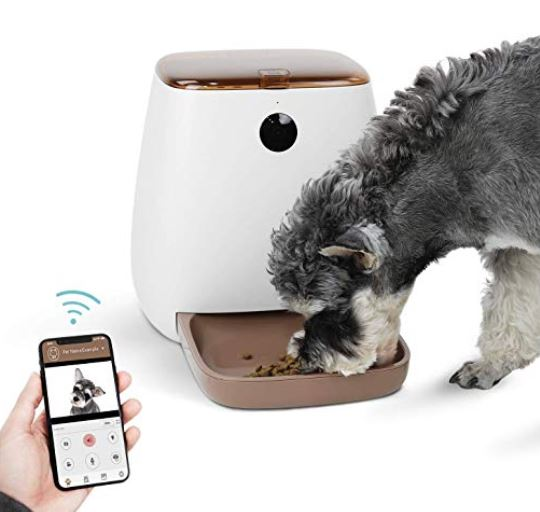
\includegraphics[width=\columnwidth]{OHANA.JPG}
  \caption{OHANA intelligent food dispenser.}\label{fig:ohana}\cite{ohana_dispenser}
\end{figure}
\begin{figure}
  \centering
  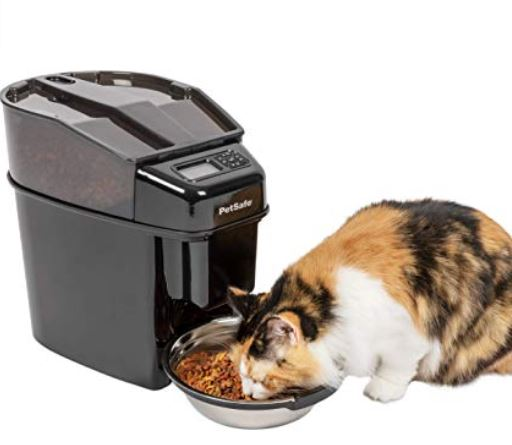
\includegraphics[width=\columnwidth]{petsafe.JPG}
  \caption{Automatic Dog and Cat Feeder by PetSafe.}\label{fig:petsafe}\cite{pet_safe}
\end{figure}




\section{Design}
The design of the automatic pet feeder consists of a physical, electrical and software design. Before starting the process of designing any of these elements the team sat down and discussed the general concepts and the main costumer need for a product of this kind and developed the CN${_0}$.  the primary requirements and  for satisfying the custumer need The primary requirement for the costumer need 



\begin{quote} \textbf{\DP1} Motor controlled auger.
\end{quote}
\begin{quote} \textbf{\DP2} Load cell.
\end{quote}
\begin{quote} \textbf{\DP3} Connected to electric outlet.
\end{quote}
\begin{quote} \textbf{\DP4} An integrated wifi chip and mobile remote or timer.
\end{quote}




As previously mentioned, using Axiomatic Design Theory is a good way to develop your design.

Here is a brief synopsis from Omarsdóttir et al.\cite{omarsdottir2016chessmate}:
\begin{quotation}
  Rather, the focus was placed on developing comprehensive FR and DP lists, then evaluating the coupling between them.
  This coupling is symbolized in a design matrix, which is a Cartesian product of all FR and DP combinations~\cite{cochran2016msdd, benevides2012aed}.
Where there is an interaction between an FR and DP, this is denoted by a non-zero coefficient, or in the case of the value being unknown, simply a placeholder variable $X$.
Minor levels of coupling, often considered higher-order effects, are annotated with $x$ to show their lessened effect.
A diagonal matrix is ``uncoupled'' and satisfies the Independence Axiom: ``to maintain the independence of the functional requirements~(FRs)''~\cite{suh2001axiomatic}.
Such a design can be easily optimized by adjusting a particular FR or DPs without affecting others.
A diagonal matrix indicates a ``decoupled'' or ``path-dependent'' solution, which can still be optimized, but the ordering of parameter choice selection becomes important.
All other design matrices are ``coupled'' and may have a usable local solution but usually resist modification and optimization~\cite{suh2001axiomatic}.
Needless to say, the focus is on minimizing coupling wherever it may appear.

ADT's second axiom is ``minimize the information content of the design.''
Simply put, ensure that the design has the highest probability of meeting the stated FRs.
When systems are not able to meet FRs all of the time, this is denoted in ADT as ``complexity'' and is deeply explored in~\cite{suh2005complexity}.
As will become apparent in the next section, this axiom became integral to the design of the interaction between the robot and its chess pieces.
Finally, any factors to be considered that are not functional are categorized as ``Constraints.''
These are often resource-focused and affect all of the design decisions; they need to be revisited often especially when choosing between otherwise equivalent implementations.
\end{quotation}
The first axiom is often called the Independence Axiom, and the second, the Information Axiom.


From the Customer Needs, we build a list of Functional Requirements.

Again, we start with a top-level \FR0: ``Contain \SI{25}{\kilogram} of fish on SureTrack conveyor until release is triggered''
From this, a top-level Design Parameter \DP0: Gable-reinforced stainless-steel locking bin with bi-directional discharge
\cite{gerhard2016suretrack}.

We continue a ``zig-zag'' procedure to decompose and map the FRs to the DPs as shown in Table~\ref{tab:first_level-frdp}.

\begin{table}
  \center
  \caption{First level FR-DP mapping.~\cite{gerhard2016suretrack}}\label{tab:first_level-frdp}
  \begin{tabular}{lll} \toprule
    ID& Functional Requirement & Design Parameter \\ \midrule 
    1&Delivers food&Motor controlled auger\\
    2&Weighable food&Load cell\\
    3&Constant power &Electric outlet/Powerbank\\
    4&Remotely controlled&WiFi chip\\
    \bottomrule
  \end{tabular}
\end{table}

From this mapping we develop a design matrix as shown in Equation~\ref{eq:top-design-matrix} from~\cite{gerhard2016suretrack}.

\begin{equation}\label{eq:top-design-matrix}
\begin{Bmatrix}
\FR{1}\\
\FR{2}\\
\FR{3}\\
\FR{4}
\end{Bmatrix}=
\begin{bmatrix}
X & 0 & X & 0\\
0 & X & X & 0\\
0 & 0 & X & 0\\
0 & 0 & X & X
\end{bmatrix}
\begin{Bmatrix}
\DP{1}\\
\DP{2}\\
\DP{3}\\
\DP{4}

\end{Bmatrix}
\end{equation}

This matrix is de-coupled i.e.\ path-dependent, meaning it can be optimized, but the order matters.

\section{Experiments}

\section{Results and Discussion}

\section{Conclusion}

\subsection{Future work}

\subsection{Summary}

%\bibliography{references}
\bibliography{references-ad}

\end{document}
%%%%%%%%%%%%%%%%%%%% TeXStudio Magic Comments %%%%%%%%%%%%%%%%%%%%%
%% These comments that start with "!TeX" modify the way TeXStudio works
%% For details see http://texstudio.sourceforge.net/manual/current/usermanual_en.html   Section 4.10
%%
%% What encoding is the file in?
% !TeX encoding = UTF-8
%% What language should it be spellchecked?
% !TeX spellcheck = en_US
%% What program should I compile this document with?
% !TeX program = pdflatex
%% Which program should be used for generating the bibliography?
% !TeX TXS-program:bibliography = txs:///bibtex
%% This also sets the bibliography program for TeXShop and TeXWorks
% !BIB program = bibtex

%%% Local Variables:
%%% mode: latex
%%% TeX-master: t
%%% End:

